% Chapter 1

\chapter{Introduction} % Main chapter title

\label{Chapter1} % For referencing the chapter elsewhere, use \ref{Chapter1} 

%----------------------------------------------------------------------------------------

% Define some commands to keep the formatting separated from the content 
\newcommand{\keyword}[1]{\textbf{#1}}
\newcommand{\tabhead}[1]{\textbf{#1}}
\newcommand{\code}[1]{\texttt{#1}}
\newcommand{\file}[1]{\texttt{\bfseries#1}}
\newcommand{\option}[1]{\texttt{\itshape#1}}

%----------------------------------------------------------------------------------------

\section{Background and Motivation}
%Overview paragraph that defines terms and big picture
Information technology costs can limit the innovation of small companies, non-profits, or municipal agencies.
Technologies like Raspberry Pi coupled with advanced software like Cassandra and Python have lowered barriers to entry for applied computing, both in terms of required knowledge and cost.
Distributed database technology like Cassandra one may associate with large data centers globally distributed, but some applications may leverage distributed systems and cloud computing principles with far less computing resources

There are many potential challenges in using Cassandra in low-cost hardware in IoT.
First, as one might expect, the computing resources are much more limited in low-cost hardware.
The Raspberry Pi 2 Model B, which will be used in this thesis, has 1GB of RAM available.  Storage for a single node depends on the SD (secure disk) card, which can vary from 8 GB to 256 GB, data rates from 2 MB/s to 30 MB/s.
These pale to the 768GB memory and 74.4 TB storage for the Lenovo Thinkserver RD650 \cite{LENOVORD650}.
Second, low cost hardware, coupled with one of many desirable applications, can imply a finite power source, powered by either a primary or secondary (rechargeable) cell.  Nothing like this limits a data center's power consumption.

\begin{figure}[h]
\includegraphics[width=15cm]{venn.png}

\caption{Venn Diagram of Application Space}

\label{fig:res}
\end{figure}


%NEED FOR DISTRIBUTED DATABASE
A distributed database offers a level of consistency, availability, and partition tolerance.  Mostly this means that a system of nodes can still operate as expected even if there is a loss of one or two nodes.

%SELECT THE REPRESENTATIVE – CASSANDRA AND WHY?
Cassandra is widely used and is known to have a high write throughput.

%DETAIL SPECS OF CASSANDRA 



%SET OF HARDWARE/OS THAT SUPPORT CASSANDRA
Cassandra specifies the “latest” versions of both “Java 8” and “Python 2.7”.  In turn, Java can run on Windows, Mac OS X, Linux, and Solaris.

\begin{table}
\begin{tabular}{ | p{3cm} | l | l | l | p{4cm} | }
  \hline

Platform & CPU Architecture & Version & Introduced In & Notes \\ \hline
%SOLARIS
%Solaris & x64 (64-bit) & 11.x & 1.8.0 & No JavaFX Support, Only 64-bit JRE is supported \\ \hline
%  Solaris & SPARC (64-bit) & 11.x & 1.8.0 & No JavaFX Support
% Only 64-bit JRE is supported \\ \hline
%Solaris & x64 (64-bit) & 10 Update 9+ & 1.8.0 & No JavaFX Support 
% Only 64-bit JRE is supported \\ \hline 
%Solaris & SPARC (64-bit) & 10 Update 9+ & 1.8.0 & No JavaFX Support 
% Only 64-bit JRE is supported \\ \hline
%WINDOWS
%Windows 10 & x86 (32-bit) & &   1.8.0\_51 \\ \hline   
%Windows 10 & x64 (64-bit) &&   1.8.0\_51  \\ \hline
%Windows 8.x & x86 (32-bit) &&  1.8.0 & Modern UI (i.e. Metro Mode) is not supported \\ \hline
%Windows 8.x & x64 (64-bit) &&   1.8.0 & Modern UI (i.e. Metro Mode) is not supported \\ \hline
%Windows 7 & x86 (32-bit)     &SP1& 1.8.0   \\ \hline
%Windows 7 & x64 (64-bit)     &SP1& 1.8.0   \\ \hline  
%Windows Vista & x86 (32-bit) &SP2& 1.8.0   \\ \hline
%Windows Vista & x64 (64-bit) &SP2& 1.8.0   \\ \hline
%WINDOWS SERVER
%Windows Server 2012 R2 & x64 (64-bit) &     & 1.8.0 \\ \hline  
%Windows Server 2012    & x64 (64-bit) &     & 1.8.0 \\ \hline  
%Windows Server 2008 R2 & x64 (64-bit) & SP1 & 1.8.0 \\ \hline  
%LINUX
%Oracle Linux & x64 (64-bit) & 7.x  & 1.8.0\_20 & Only 64-bit JRE is supported \\ \hline 
%Oracle Linux & x86 (32-bit) & 6.x  & 1.8.0   \\ \hline 
%Oracle Linux & x64 (64-bit) & 6.x  & 1.8.0 & Only 64-bit JRE is supported \\ \hline 
%Oracle Linux & x86 (32-bit) & 5.5+ & 1.8.0 & No JavaFX Support \\ \hline 
%Oracle Linux & x64 (64-bit) & 5.5+ & 1.8.0 & No JavaFX Support \\ \hline 
%Red Hat Enterprise Linux & x64 (64-bit) & 7.x & 1.8.0\_20 & Only 64-bit JRE is supported \\ \hline 
%Red Hat Enterprise Linux & x86 (32-bit) & 6.x & 1.8.0 \\ \hline 
%Red Hat Enterprise Linux & x64 (64-bit) & 6.x & 1.8.0 & Only 64-bit JRE is supported \\ \hline 
%Red Hat Enterprise Linux & x86 (32-bit)     & 5.5+ & 1.8.0 & No JavaFX Support \\ \hline 
%Red Hat Enterprise Linux & x64 (64-bit)     & 5.5+ & 1.8.0 & No JavaFX Support \\ \hline 
%Suse Linux Enterprise Server & x64 (64-bit) & 12.x & 1.8.0\_31 & Only 64-bit JRE is supported \\ \hline 
%Suse Linux Enterprise Server & x86 (32-bit) & 11.x    & 1.8.0   \\ \hline 
%Suse Linux Enterprise Server & x64 (64-bit) & 11.x    & 1.8.0   \\ \hline 
%Suse Linux Enterprise Server & x86 (32-bit) & 10 SP2+ & 1.8.0 &  gtk2 2.18+ is required for supporting JavaFX \\ \hline 
%Suse Linux Enterprise Server & x64 (64-bit) & 10 SP2+ & 1.8.0 &  gtk2 2.18+ is required for supporting JavaFX \\ \hline 
%Ubuntu Linux & x86 (32-bit) & 15.10 & 1.8.0\_65   \\ \hline 
%Ubuntu Linux & x64 (64-bit) & 15.10 & 1.8.0\_65   \\ \hline 
%Ubuntu Linux & x86 (32-bit) & 15.04 & 1.8.0\_45   \\ \hline 
%Ubuntu Linux & x64 (64-bit) & 15.04 & 1.8.0\_45   \\ \hline 
%Ubuntu Linux & x86 (32-bit) & 14.x  & 1.8.0\_25   \\ \hline 
%Ubuntu Linux & x64 (64-bit) & 14.x  & 1.8.0\_25   \\ \hline 
%Ubuntu Linux & x86 (32-bit) & 13.x  & 1.8.0   \\ \hline 
%Ubuntu Linux & x64 (64-bit) & 13.x  & 1.8.0   \\ \hline 
%Ubuntu Linux & x86 (32-bit) & 12.04 - LTS & 1.8.0   \\ \hline 
%Ubuntu Linux & x64 (64-bit) & 12.04 - LTS & 1.8.0   \\ \hline 
%LINUX ON ARM
Ubuntu Linux
 (Hard-Float ABI) & ARMv8     & 14.04 - LTS & 1.8.0\_60 & No JavaFX Support  \\ \hline 
Ubuntu Linux
 (Hard-Float ABI) & ARMv7 VFP & 12.04 - LTS & 1.8.0     & No JavaFX Support \\ \hline 
%OS X
%OS X & x64 & 10.9 and above & 1.8.0 & Only 64-bit JRE is supported \\ \hline 
%OS X & x64 & 10.8.3+        & 1.8.0 & Only 64-bit JRE is supported \\ \hline 

\end{tabular}
\caption{Oracle JDK 8 and JRE 8 Certified System Configurations, ARM \cite{OracleOracleConfigurations}}
\end{table}


%SELECT THE REPRESENTATIVE – RASPBERRY PI, FOR NOW

%TRANSITION


\subsection{Potential Uses}
\subsubsection{Application Space figure and explanation}
\subsubsection{WiFi Collection, mapping and analytics}
WiFi sniffing, or war-driving, has been explored by a number of enthusiasts.
For instance, Snoopy \cite{SensePostFramework} provides a framework for collecting WiFi data and observing with Maltego.
In addition, one can sniff wireless traffic by using software Aircrack-ng \cite{Aircrack-ng} or Airsnort \cite{AirSnortHomepage}.
%\subsection{WiFi Mapping}
There has been much work done with respect to WiFi mapping.  Argos \cite{Rose2010MappingArgos} describes a similar system of a distributed system, but there is no mention of Cassandra or any distributed database, which may serve as an improvement on such a sensor network.  Wigle.net \cite{WiGLE:Mapping} is an aggregate map that distributes a smart-phone application to collect GPS coordinate-Access Point pairs, but relies on a central database, and has an unreliable user base and irregular sampling frequencies (relying on the public).  It is also worth noting that records are not updated.  Heat Mapper \cite{HeatMapperOffices} is partially free and commercial software that can generate a heat map for a small room or office.  Wi2Me \cite{Castignani2012Wi2Me:Networks} performs this mapping as well, with an emphasis on performance and data throughput.  It uses an instance of SQLite to store the traces on the individual's smart-phone, but again, none of these make use of a distributed database like Cassandra as part of the sensor network.

%\subsubsection{WiFi/Wireless Crowd Detection}
There are numerous blog posts that lay claim to the fact that individuals are tracked via commerical entities via WiFi \cite{HaighTrackingConnected}. Some have reported to make art exploiting this mechanism \cite{KeebleCasual2013}.

There have been efforts to track crowds, notably \cite{Bonne2013WiFiPi:Events} and \cite{Schauer2014EstimatingBluetooth}.  
\subsubsection{CBIR and others and summary statement on application space}


\subsection{Representative Technologies}

\subsubsection{Cassandra}
\label{Cassandra}
Cassandra is a widely used distributed \gls{nosql} database with many use cases \cite{Lakshman2010CassandraSystem}.
Not only has Cassandra been reportedly been used in practice \cite{ApacheCases}, but has been, using the Yahoo Cloud Services Benchmark \cite{YahooBenchmark}, formally evaluated in scholarly literature against other databases such as MongoDB and proposed as the NoSQL database of choice in the Internet of Things and distributed sensor networks \cite{Abramova2013NoSQLCassandra}.
There have been credible claims of Cassandra being used on Raspberry Pi \cite{VanRyswykMulti-DatacenterPis,SercelCassandraMedium}, but to the author's knowledge, no white paper with the details exists.
%But in a way, this is the simplified version of the application that this is testing.
The aim of this paper is to examine Cassandra's performance coupled with a simplified Wi-Fi collection and analysis application, where the nature of link nodes may be less reliable than wired Ethernet.

This author's interest in Cassandra lies in the fact that Cassandra is a distributed database used in practice for cloud computing.
Although it describes itself as a NoSQL database, the interface allows for SQL commands and has a Python API.
Cassandra allows for configuration of distributed systems parameters, such as replication factor, but detailed knowledge of distributed systems protocols is not critical for operation.

From an experimental standpoint, the distributed nature of a Cassandra "keyspace" lies in four parameters \cite{CassandraDummies}: cluster size (the number of nodes), replication factor (configured in software), write level (configured in software), and read level (configured in software).
As alluded to in section \ref{Factors Held Constant}, these factors will be held constant for this experiment.

\cite{Bonne2013WiFiPi:Events} goes over \gls{gsm} to a central node, but does not use any kind of distributed database, like Cassandra.  There are commercial entities that claim to track crowds and report data, namely Bluemark \cite{SchiphorstBlueInnovations}.  Here as well, a central server is utilized to collect the data.
Users then reportedly log into the web to view the metrics.  According to their marketing literature, they do use Raspberry Pi, but not for data storage.
Paper \cite{ChilipireaPresumablyWiFi} used this product line for their tests.

Although WiFi utilizes \gls{mac} addresses supposedly unique to each device, research has found that this is not always suitable or reliable for many applications, namely crowd-tracking.  For instance, some devices have been reported to change their MAC addresses \cite{ChilipireaPresumablyWiFi}.  There exist a number of papers that talk about and look into characterizing mobile devices and their users at the individual level \cite{Pang2007802.Fingerprinting} \cite{Chernyshev2016ServiceChallenges} \cite{Cunche2014LinkingRequests} \cite{Du2016EV-Linker:Matching} \cite{Cunche2012IRequests} \cite{Luzio2016MindRequests} \cite{Musa2012TrackingMonitors} and propose techniques to better prepare data for analysis \cite{ChilipireaPresumablyWiFi}.  In all of these, however, distributing the data among the nodes, like with Cassandra is either not used or not mentioned.  Many utilize a central server that represents a single point of vulnerability.




\subsubsection{Raspberry Pi 2}

The Raspberry Pi 2 (Model B) \cite{RaspberryB} is a low-cost computer designed sold from the United Kingdom.
It can be described as a motherboard for a about the size of a 3x5 index card and has been available since February 2015.
This experiment is interested in the Raspberry Pi 2 as a representative of the low-cost hardware domain, which implies low cost, low power consumption, and low in terms of size and weight.

This author's interest in the Raspberry Pi 2 is that its ARM Cortex-A7 processor and 1GB RAM \cite{RaspberryB} makes it a key representative of the low-cost hardware domain and the Internet of Things.
The Raspberry Pi 2 has cost as low as 35 USD \cite{RaspberryPi}.
It is lightweight and has limited power consumption \cite{RaspberryB}.
Constraints on size, weight, power, and cost can all be barriers to entry for applications seeking computing nodes.

Expanding this experiment, to say the BeagleBone black \cite{BeagleBoard.orgBlack}, is in touch with the spirit of this experiment but outside the scope of this paper.
See section \ref{Conclusion} for elaboration on future work.

%\subsection{Wireshark software and PCAP files}

%A PCAP file stores networking packets and is a "main capture file format" \cite{tcpdumpTcpdump/LibpcapRepository}.
%In this case, the PCAP file is used as a tool in the benchmark, a means to an end.

%Commonly associated with PCAP files, and used by this author is the Wireshark software \cite{WiresharkDeep.}.
%This was used to view and confirm that the PCAP files were generated to taste.

%Not even a vague familiarity of these is needed to understand the experiment, but they are a fundamental part of the custom benchmark of choice. 



\section{Problem Statement and Research Goals}

%Paragraph 1 – Problem Statement
\subsection{Problem Statement}
To gauge expectation in the variation in how modern distributed databases operate in an \gls{iot} environment, where applications that call or benefit from an open-source distributed database, and what actions or configurations may be required or recommended to be in place for this to happen.
%Paragraph 2 – General Approach 
\subsection{General Approach}
%                Sentence 1,2,&3 – 
% As of now, this was directly from JP
The general approach to this will be to implement a scientific methodology for understanding the effect of inherent aspects of \gls{iot} networks on factors that limit performance of distributed databases. We are particularly interested in the effects of low memory and processor speed, limited bandwidth and scalability on IoT networked devices. In general, this study follows a template that includes varying configuration and environment settings, performing stress testing, measuring results, and interpreting the results to form a conclusion.                 
% Paragraph 3 – Research Activity Overview (1-2 sentences)
\subsection{Research Activity Overview}
This paper will apply the \gls{ycsb} benchmarking tool to gauge performance changes over variation in the following: keyspace configuration, network configuration, platform choice, and node scaleup.
%Sub-bullet 1 – Sensitivity Testing
\subsubsection{Sensitivity Testing}
Cassandra, like other distributed databases, can be configured or "tuned" to suit the application.
For instance, one can tune the cache parameters of a Cassandra keyspace.
It may be desirable to know, as the hardware capabilities go down, does this have a proportional or more-than-proportional effect on how application performance sensitivity.
%Sub-bullet 2 – Bandwidth testing
\subsubsection{Bandwidth Testing}
For many applications, it is desirable to move toward wireless applications.

%Sub-bullet 3 – Platform testing
\subsubsection{Platform Testing}
There are a lot of factors that can go into switching hardware: \gls{cpu}, \gls{ram}, and \gls{io} interfaces.

%Sub-bullet 4 – Scalability testing
\subsubsection{Scalability Testing}
% Paragraph 4 – Research Activity Summary (1-2 sentences)
A common selling point for distributed databases is an ability to accept additional nodes for storage, as opposed to say, more storage in-situ.

\section{Expected Contributions}
\subsection{Expected Contributions Overview}
%Paragraph 1 – Expected Contributions Overview (1-2 sentences)
This paper is expected to contribute a few points for the reader.
\subsubsection{Contribution 1}
First, this paper develops a methodology to limit existing tools \cite{YahooBenchmark} to evaluate a NoSQL distributed database in \gls{iot}.
%Sub-bullet 1 – Contribution 1
\subsubsection{Contribution 2}
This will expand on such work as \cite{Abramova2014TestingCassandra} and \cite{YahooBenchmark} developing a test methodology to explore the limits of Cassandra, and how its performance is affected by the number of nodes, nature of hardware, and links.
%Sub-bullet 2 – Contribution 2
\subsubsection{Contribution 3}
This paper will also briefly depart from the laboratory mindset in order to demonstrate potential applications in \gls{iot}.
%Sub-bullet 3 – Contribution 3
\subsection{Expected Contributions Summary}
%Paragraph 2 – Expected Contributions Summary (1-2 sentences)


\section{Thesis Organization}

\begin{figure}[h]
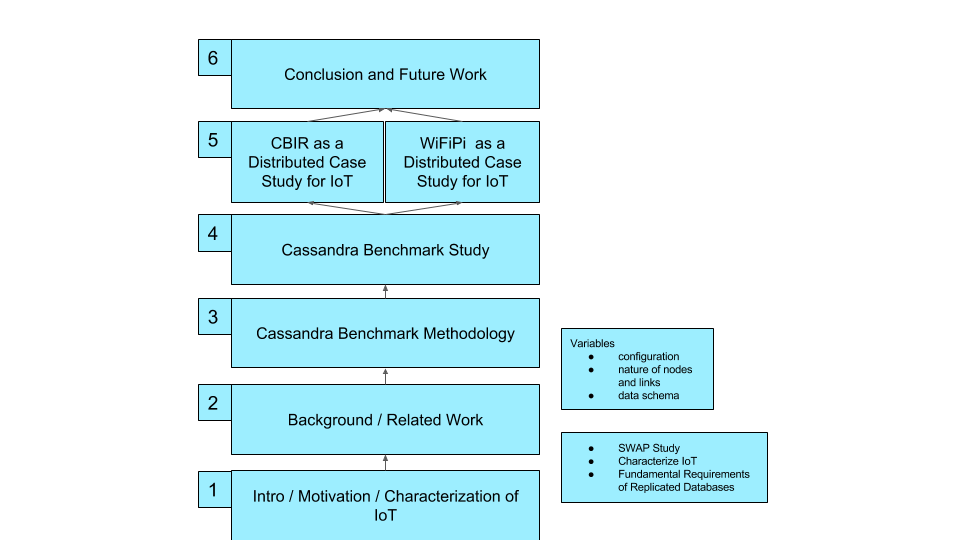
\includegraphics[width=15cm]{thesis_organization.png}

\caption{Thesis Organization}

\label{fig:res}
\end{figure}

	Aggregating lower-cost, lightweight hardware spawns a lingering question of possibilities and performance due to lower barriers to proliferation.  This first Chapter explored the motivation and background of \gls{iot} applications that require distributed, high availability data. With distributed database Cassandra representative of application, and the Raspberry Pi a representative of low-cost hardware, we explore the performance of a distributed database over Raspberry Pi networked clusters. 

Chapter 2 describes the background in greater detail. There are many papers that put Cassandra to the test, but literature is few and far between for low cost hardware like the Raspberry Pi 2. We also present the gaps of the current literature to describe the technical goals for the current work.
	
Chapter 3 presents an investigation of both nondeterministic and deterministic variation with respect to performance measurements, such as read and write latency.  Deterministic variation can come in three basic categories: hardware (processor model, RAM, networking hardware, protocols, topology), Cassandra’s configuration (partitioner, commit log total space), and the nature of the keyspace (data schema, replication strategy, etc.). Chapter 4 describes the implementation of the methodology presented in Chapter 3, revealing a sensitivity analysis.  
	
In order to give the benchmarking study due relevance, two case studies in Chapter 5 place the benchmarking in comparison to applications in development.  First, we show a distributed streaming application for wireless sniffing as a case study for IoT using Cassandra. The study, patterned off of WiFiPi[cite] is an example of distributed sensing and storage that can be applied to detect open 802.11a/b/g/n signals to gain general situational awareness.  We investigate when Cassandra is working in conjunction with a sensing application.  Second, we show a content based image retrieval application that uses Cassandra on IoT devices for a distributed surveillance application. Images represent a significant data and processing load.  We investigate the Cassandra’s performance when working in conjunction with cloud computing over low-cost hardware. 
	
WiFiPi is an example of distributed sensing and storage that can be applied to detect open 802.11a/b/g/n signals to gain general situational awareness.  We investigate when Cassandra is working in conjunction with a sensing application.
In Chapter 6, this study is brought to a conclusion and future work is discussed.





